\documentclass[11pt,aspectratio=169]{beamer}
\usetheme{Madrid}
 
% ---------- Micro-typography ----------
\usepackage[expansion=false]{microtype}
 
% ---------- Math & symbols ----------
\usepackage{mathtools}          % includes amsmath
\usepackage{amssymb,amsfonts}
 
% ---------- Graphics / colors / tables ----------
\usepackage{graphicx}
\usepackage[table]{xcolor}      % includes colortbl
\usepackage{float}              % [H] placement for figures
 
 
% ---------- Bibliography ----------
\usepackage{natbib}
 
% ---------- Misc ----------
\usepackage{etoolbox}
\pdfstringdefDisableCommands{\def\translate#1{#1}}
 
 
% ==================================================
%                 COLOR PALETTE
% ==================================================
 
\definecolor{darkpink}{RGB}{139,0,75}
\definecolor{lightsoftpink}{RGB}{250,225,235}
 
 
% ==================================================
%              BEAMER LOOK-AND-FEEL
% ==================================================
 
% Frame titles
\setbeamercolor{frametitle}{fg=white,bg=darkpink}
\setbeamertemplate{frametitle}{%
  \nointerlineskip%
  \begin{beamercolorbox}[wd=\paperwidth,ht=3ex,dp=1.5ex,leftskip=0.7cm]{frametitle}
    \insertframetitle
  \end{beamercolorbox}%
}
 
% Structure color (bullets, numbering, etc.)
\setbeamercolor{structure}{fg=darkpink}
 
% Background
\setbeamercolor{background canvas}{bg=white}
 
% Blocks
\setbeamercolor{block title}{bg=darkpink,fg=white}
\setbeamercolor{block body}{bg=lightsoftpink,fg=black}
 
% Remove footline
\setbeamertemplate{footline}{}
\addtobeamertemplate{title page}{\vspace*{-0.5\baselineskip}}{}
 
 
% ==================================================
%               CONVENIENCE
% ==================================================
 
\setbeamertemplate{itemize items}[circle]
\setbeamertemplate{itemize subitem}{\tiny\raise1.5pt\hbox{\donotcoloroutermaths$\color{darkpink}\blacktriangleright$}}
\setbeamertemplate{itemize subsubitem}{\scriptsize\raise1.5pt\hbox{\donotcoloroutermaths$\color{darkpink}\bullet$}}
 
% ---------- Figure source note ----------
\newcommand{\source}[1]{\vspace{-0.5em}\par\footnotesize\textit{Source:} #1}
 
% Margins
\setbeamersize{text margin left=2em, text margin right=2em}
\addtolength{\leftmargini}{2em}
 
 
%%%%%%%%%%% ------ TITLE PAGE --------- %%%%%%%%%%%%%%%%%%%
\title{Does Female Leadership Relate to Productivity-Wage Gaps in Colombia? \\
{\small Applied Microeconomic Theory ECON 6301 Paper}}
\author{Ingri Katherine Quevedo Rocha}
\institute{\small \url{ingriq@gwu.edu} \\ George Washington University \\ M.S.\ Applied Economics (Spring 2026)}
\date{\today}
 
 
%%%%%%%%%%%%%%%%%%%%%%%%%%% BEGIN %%%%%%%%%%%%%%%%%%%%%%%
\begin{document}
 
\begin{frame}
  \titlepage
\end{frame}

%%%%%%----------------------%%%%%%
\begin{frame}{Introduction}

\textbf{This paper examines whether female leadership (measured as the share of female executives) attenuates the productivity-wage gap.}
\vspace{0.2em}
\begin{itemize}
  \item Across the world, workers are paid substantially less than the value they produce. Eg: Colombia workers receive about 40\% of their contribution to production.
  \item This occurs due to labor market frictions and imperfections, where firms have some degree of monopsony power over workers.
  \item Still, firms differ substantially in how aggressively they exploit it, and management choices shape wage-setting and competition.
  \item Literature suggests that female leaders place greater weight on worker welfare and are less likely to engage in anticompetitive behavior.
\end{itemize}

\end{frame}


%%%%%%----------------------%%%%%%

\begin{frame}{Results}
\vspace{-0.5em}
\begin{columns}[T]
    \begin{column}{0.55\textwidth}
    \begin{equation*}
    \begin{split}
        \log(\text{Markdown}_{it}) &= \alpha + \beta \, \text{FemaleLeadership}_{it} \\
                                   &\quad + \boldsymbol{\gamma}' \mathbf{X}_{it} + \alpha_t + \alpha_s + \alpha_r + \varepsilon_{it}
    \end{split}
    \end{equation*}
    \vspace{0.2em}
    {\small $\hat{\beta} \approx -0.001$: A 10 percentage-point increase in the share of female executives is associated with a 1\% decrease in the markdown, holding all else constant. \\
    Economic magnitude: This corresponds to a decline in the median markdown from 1.680 to about 1.662, increasing the worker's share from \$59.5 to \$60.2 for every \$100 produced.}
    \end{column}
    \begin{column}{0.45\textwidth}
    \centering
    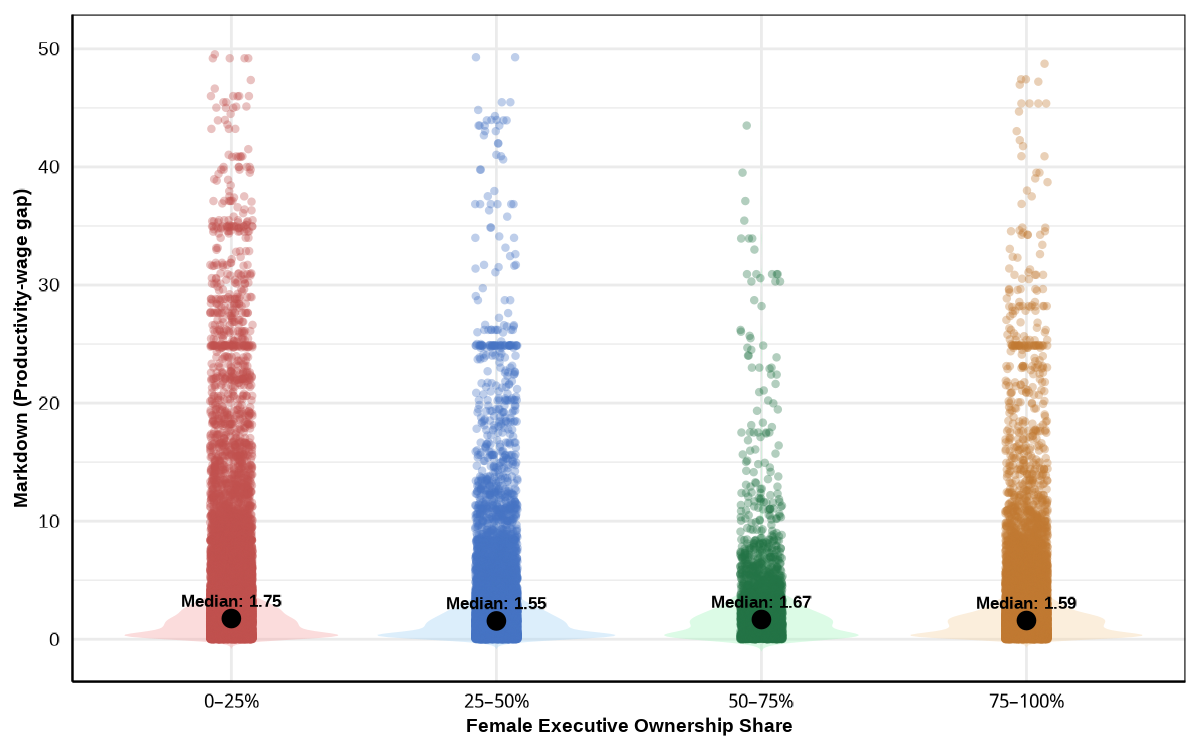
\includegraphics[width=\textwidth, height=0.62\textheight, keepaspectratio]{violin_markdown_ownwshare.png}
    \par\vspace{0.3em}
    {\small\textbf{Figure:} Markdown and Female Leadership}
    \par{\tiny Source: Author's calculations based on the Colombian Manufacturing Survey (EAM), 2000--2019.}
    \end{column}
\end{columns}
\end{frame}
\end{document}